\section{Geometry and Textures}

Geometry plays a fundamental role in CG. At the start, we need to define how we want to represent geometry in a discrete setting. Source data can be acquired by 3D scanning, digital modelling, procedural modelling, etc. We mainly differentiate by data generated on a computer (mesh) vs. data acquired from real-world object (point cloud).


\subsection{Geometry Representation}
 
If we look at geometry representation, we need to think about storage, acquisition / creating of shapes, editing of shapes and rendering of shapes. \medskip

\textbf{Parametric Surfaces} are surfaces that are defined by a parameter space. This allows us to simplify the storage to the position in the parameter space. On the downside, if there is no parameterisation of a surface, this does not work. \medskip

\textbf{Subdivision Surfaces} are surfaces that are piecewise linear. By increasing the subdivision, we can increase the number of surfaces and the precision. \medskip

\textbf{Point Set Surfaces} are a collection of points that can be combined to surfaces. \medskip

\textbf{Polygonal Meshes} store the boundary of objects and the connectivity.
\begin{center}
	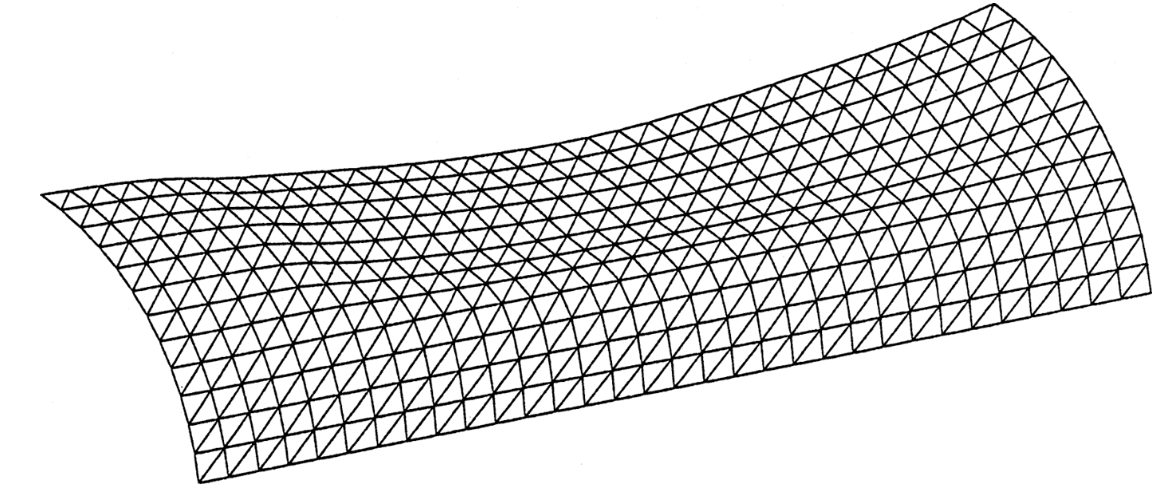
\includegraphics[width=0.9\linewidth]{mesh.png}
\end{center}

Todays GPU pipelines are optimized for such mesh structures and therefore provide fast rendering. On a mathematical level we define a polygon by a set of vertices $V = \{v_0, ..., v_{n-1}\}$ and a set of edges $E = \{(v_0, v_1), ..., (v_{n-2}, v_{n-1})\}$. A polygon is planar and non-self-intersecting. \medskip

A polygonal mesh is a set of connected polygons $M = (V, E, F)$ where $F$ are the faces of the polygons. It has the following properties:
\begin{itemize}
	\item Every edge belongs to at least one polygon
	\item The intersection of two polygons in $M$ is either empty, a vertex, or and edge
\end{itemize}

A manifold is a surface locally homeomorphic to a disk.
\begin{center}
	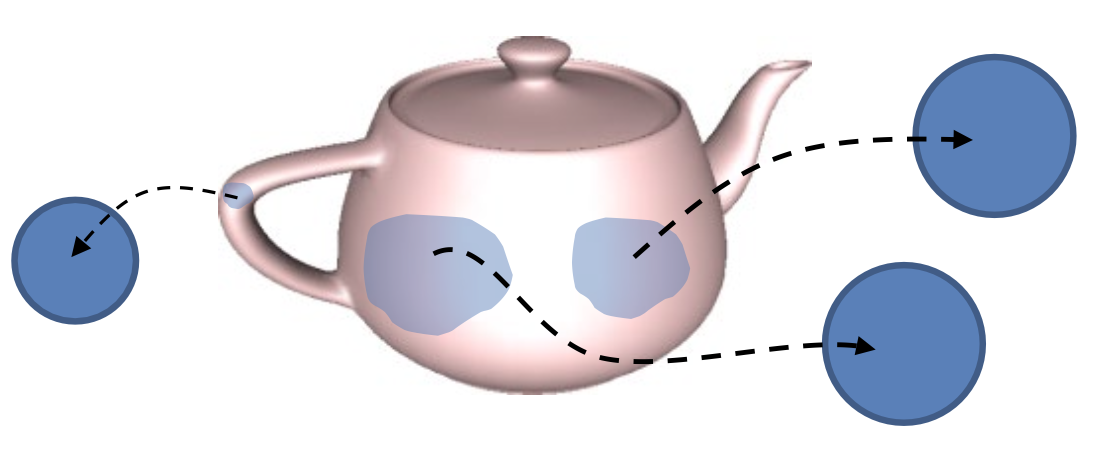
\includegraphics[width=\linewidth]{manifold.png}
\end{center}

In a manifold mesh there are some structures that are not allowed:
\begin{center}
	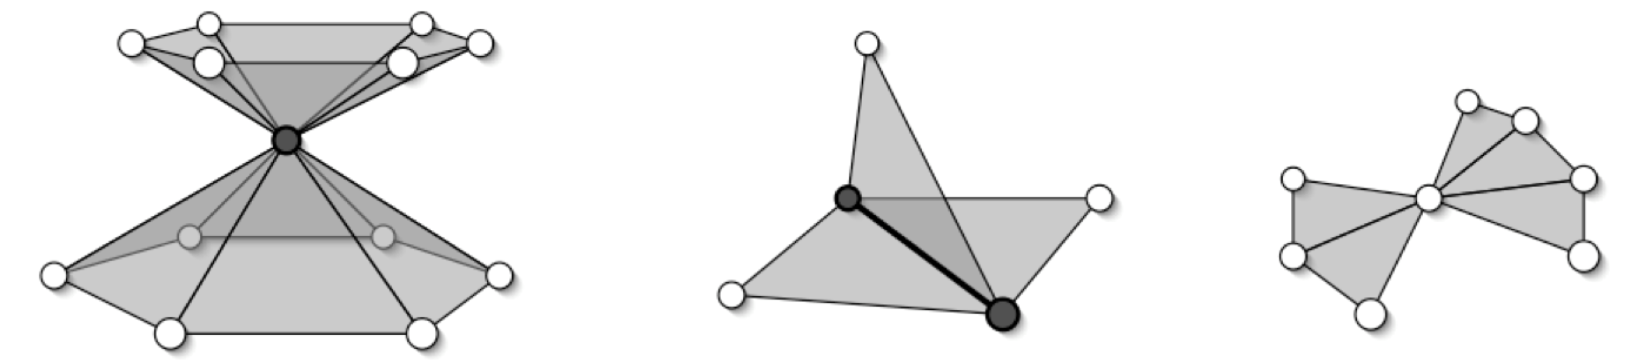
\includegraphics[width=\linewidth]{non_manifold.png}
\end{center}

Real-world data is often non-manifold.


\subsection{Mesh Data Structures}

We want to store the geometry and topology of a polygonal mesh. This data structure should allow for easy rendering, support geometry queries and allow for modifications. \medskip

\textbf{Triangle Lists} are a simple data structure. On the downside, they do not provide information about connectivity and are largely redundant (vertex gets saved multiple times).
\begin{center}
	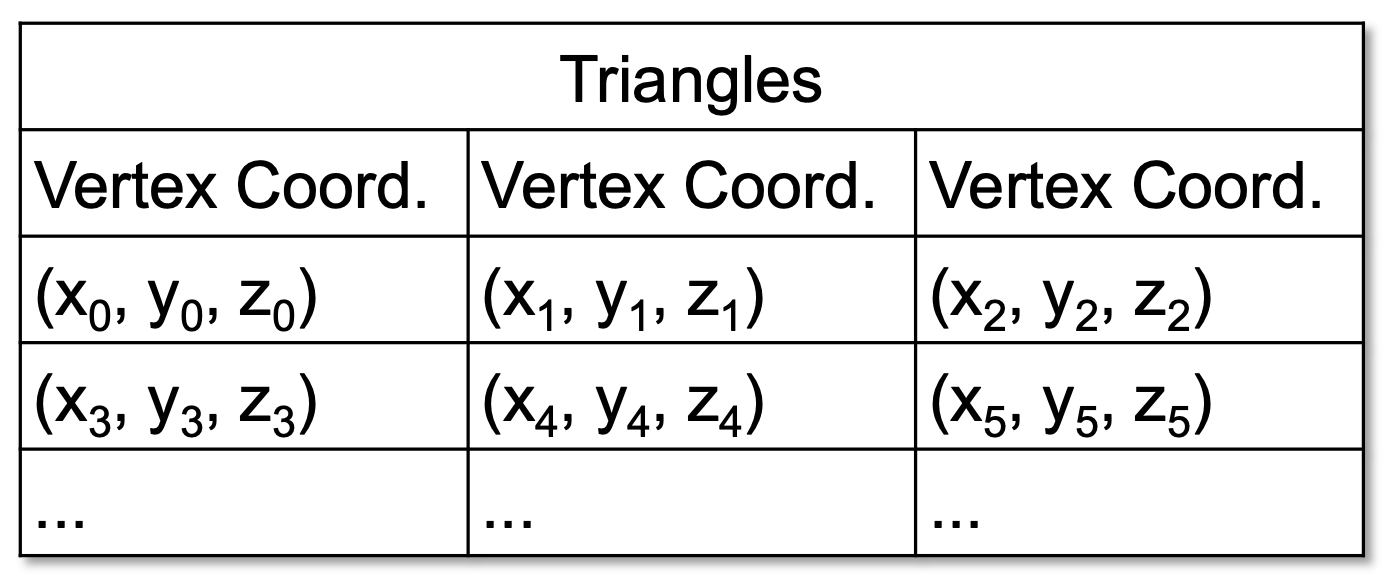
\includegraphics[width=0.65\linewidth]{triangle_list.png}
\end{center}

\textbf{Indexed Face Set} are a lot more efficient, store connectivity and eliminate the redundancy. On the other hand geometric queries and modifications are costly.
\begin{center}
	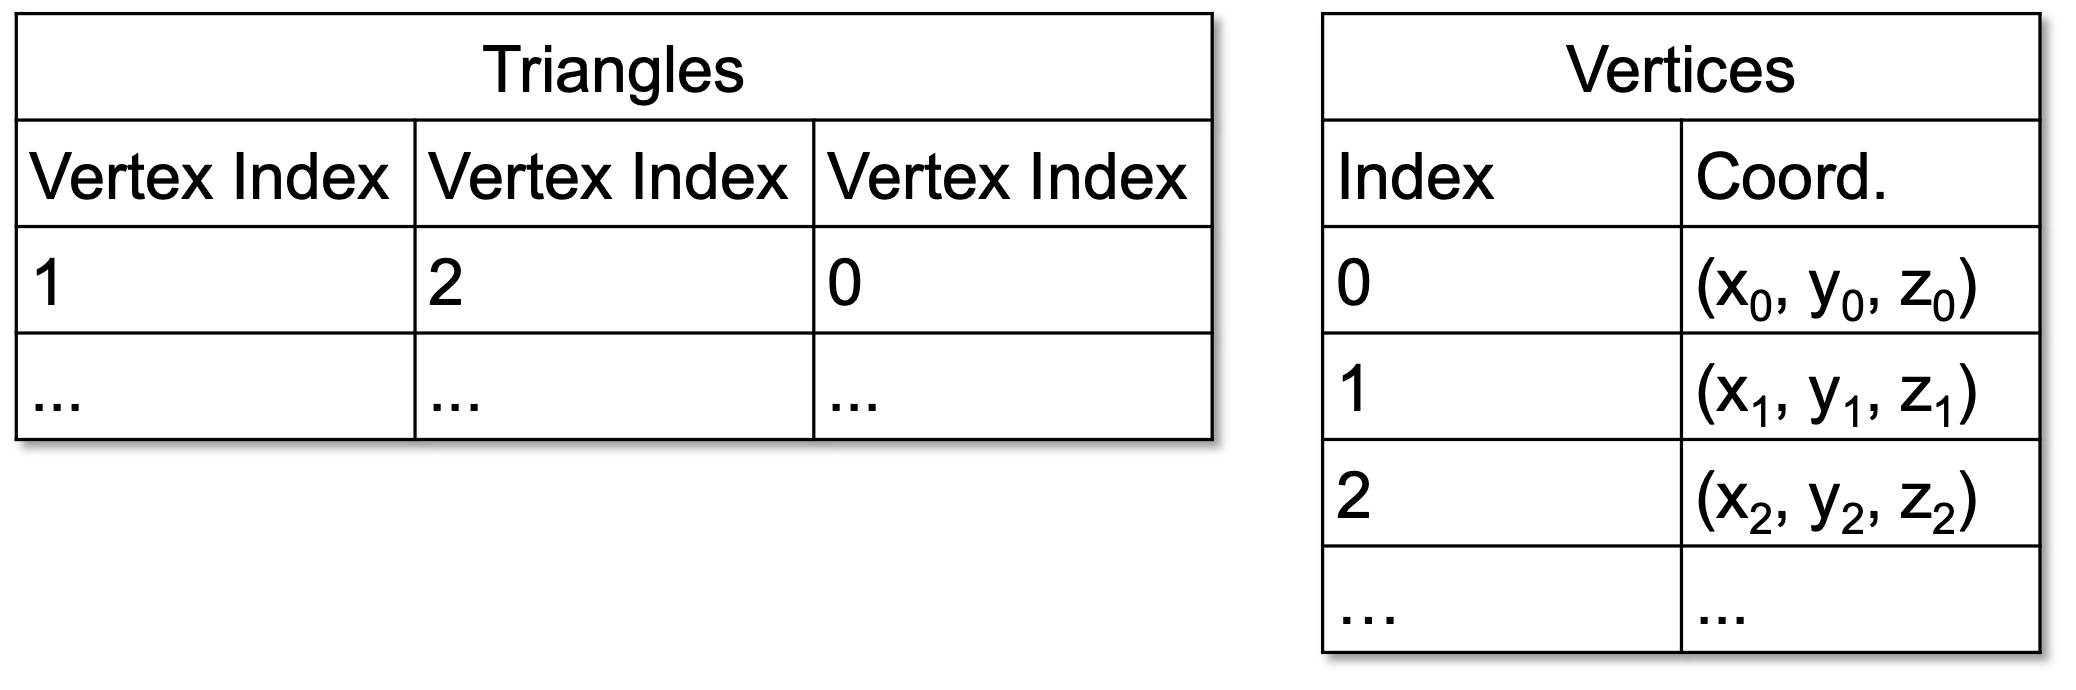
\includegraphics[width=\linewidth]{indexed_face_set.png}
\end{center}


\subsection{Texture Mapping}

On fundamental way to enhance the quality of our renderings are texture mapping. Texture mappings increase the level of detail, without increasing our geometric mesh.
\begin{center}
	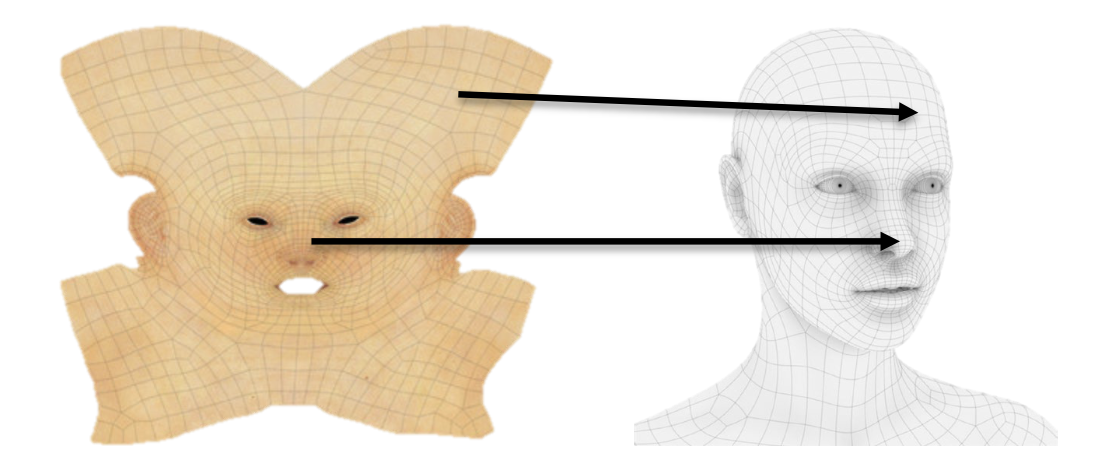
\includegraphics[width=\linewidth]{texture_map.png}
\end{center}

The difficulty is to find this mapping (2D to 3D space), this can lead to aliasing, blur or level-of-detail issues. \medskip

Texture mapping creates a one-to-one mapping between the texture and the geometry, this is done by parameterization of our geometric surface. We want the mapping to have the following properties:
\begin{itemize}
	\item Low Distortion
	\item Bijective Mapping
	\item Efficient to Compute
\end{itemize}

Finding a good texture map can be done by using a texture atlas or by finding cuts to transform our 3D surface into 2D. 


\subsection{Texture Filtering}

When we project our texture to a surface it is subject to aliasing.
\begin{center}
	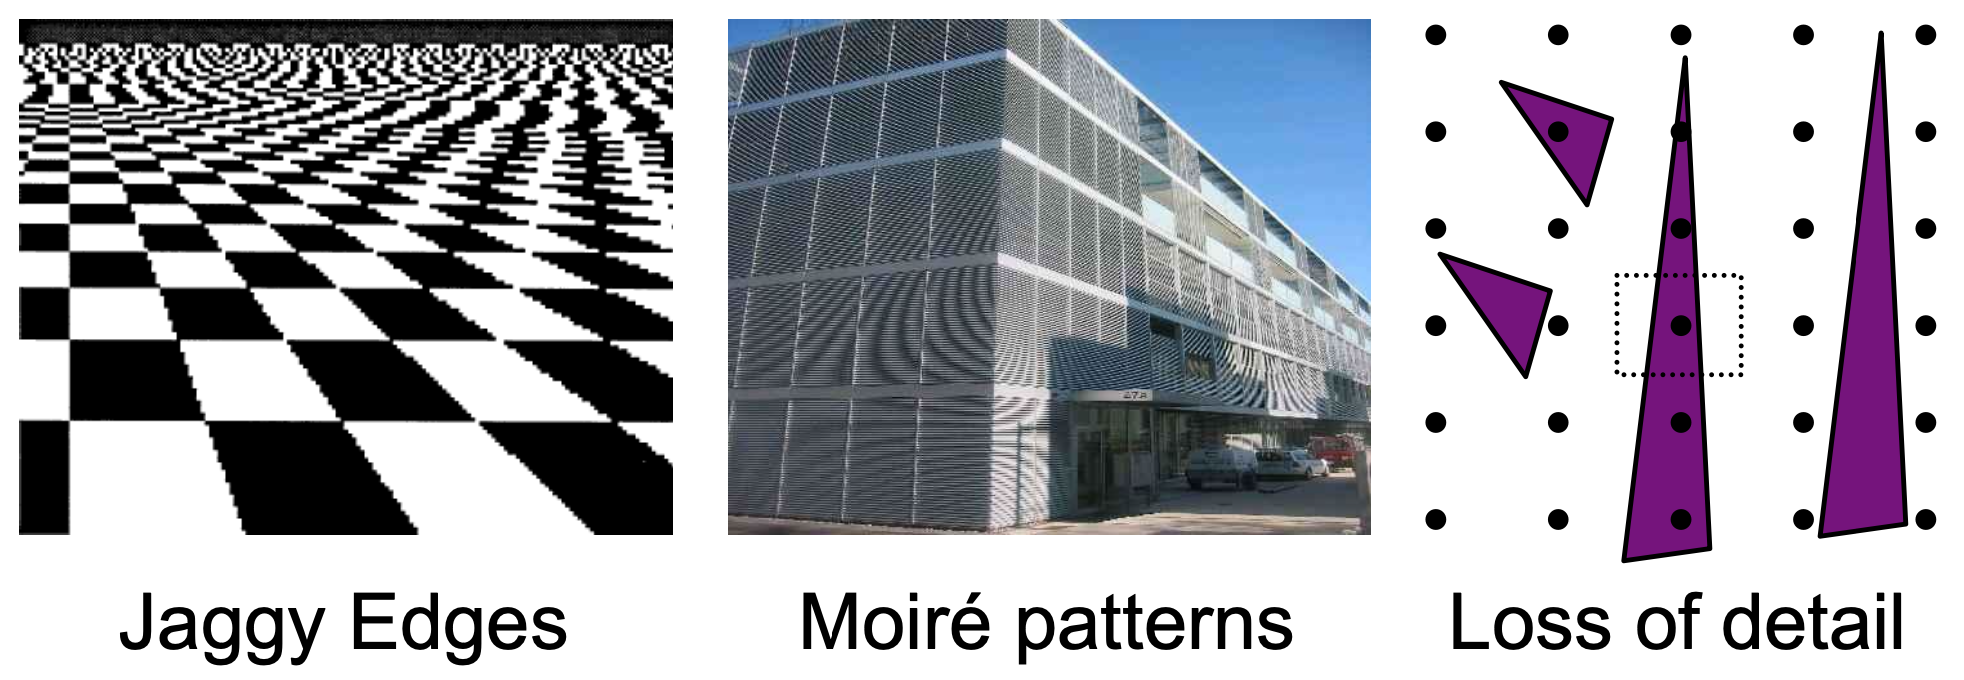
\includegraphics[width=\linewidth]{texture_filtering.png}
\end{center}

Low-pass filtering can help us avoid this aliasing. A typical low-pass filter would be the Gaussian filter. \medskip

Filtering in texture space is different form filtering in screen space. If we have an isotropic Gaussian in screen space this can relate to an anisotropic Gaussian in texture space.
\begin{center}
	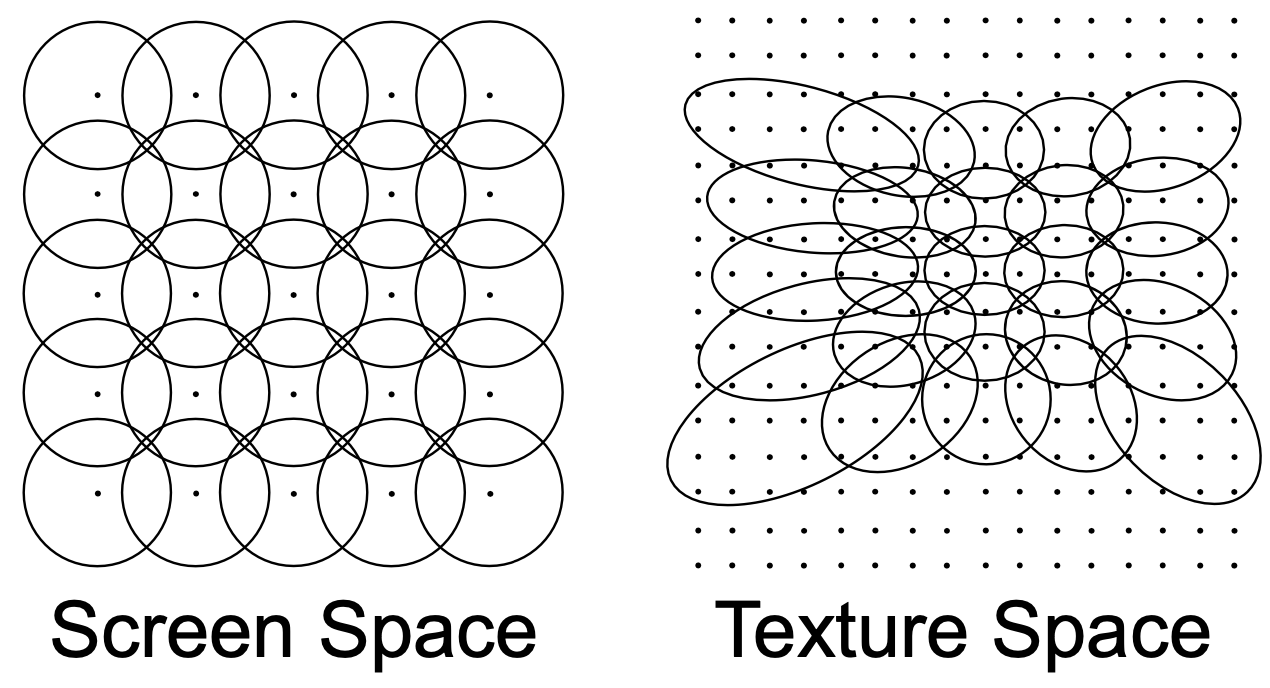
\includegraphics[width=0.9\linewidth]{filtering.png}
\end{center}


\subsection{Light Map}

Light maps are a trick to simulate the effect of a local light source.
\begin{center}
	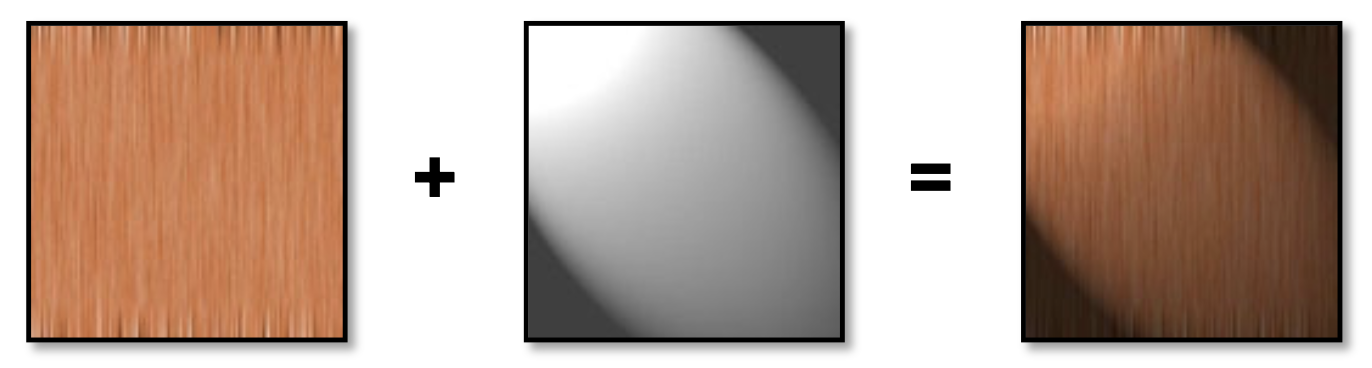
\includegraphics[width=\linewidth]{light_map.png}
\end{center}

They allow for fast and high-quality shadows and lighting with an unlimited amount of light sources. On the downside they are not suited for every lighting model, take up space, do not work with moving light and take a lot of time to generate.


\subsection{Environment Map}

Environmental maps are used to render reflective objects efficiently. It works by by intersecting the reflected ray with the surrounding sphere or cube map.
\begin{center}
	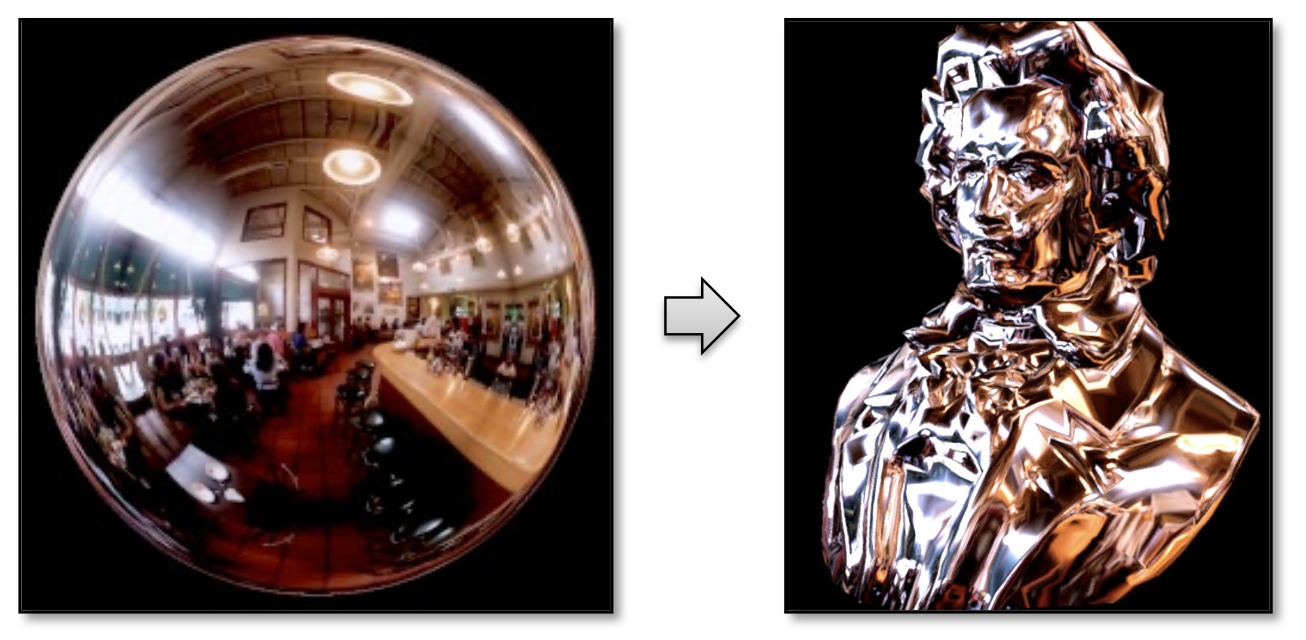
\includegraphics[width=\linewidth]{environment_map.png}
\end{center}


\subsection{Bump Mapping}

Bump maps are used to perturb surface normal according to textures, allowing us to represent small-scale geometry (e.g. pores).
\begin{center}
	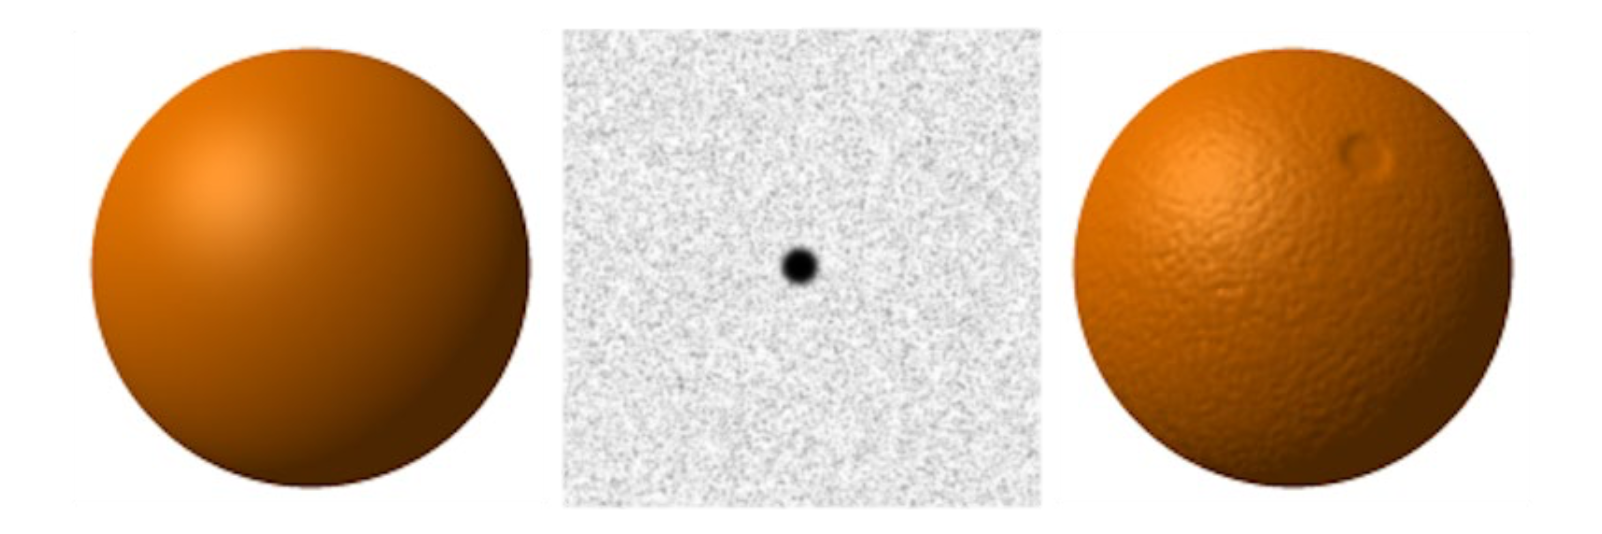
\includegraphics[width=\linewidth]{bump_map.png}
\end{center}

One limitation of bump mapping is that it does not work on the silhouette.


\subsection{Procedural Textures}

Combining Perlin noise (or other types of noise) in different resolutions, allows us to create procedural textures. One examples for such a texture would be wood textures.

\begin{center}
	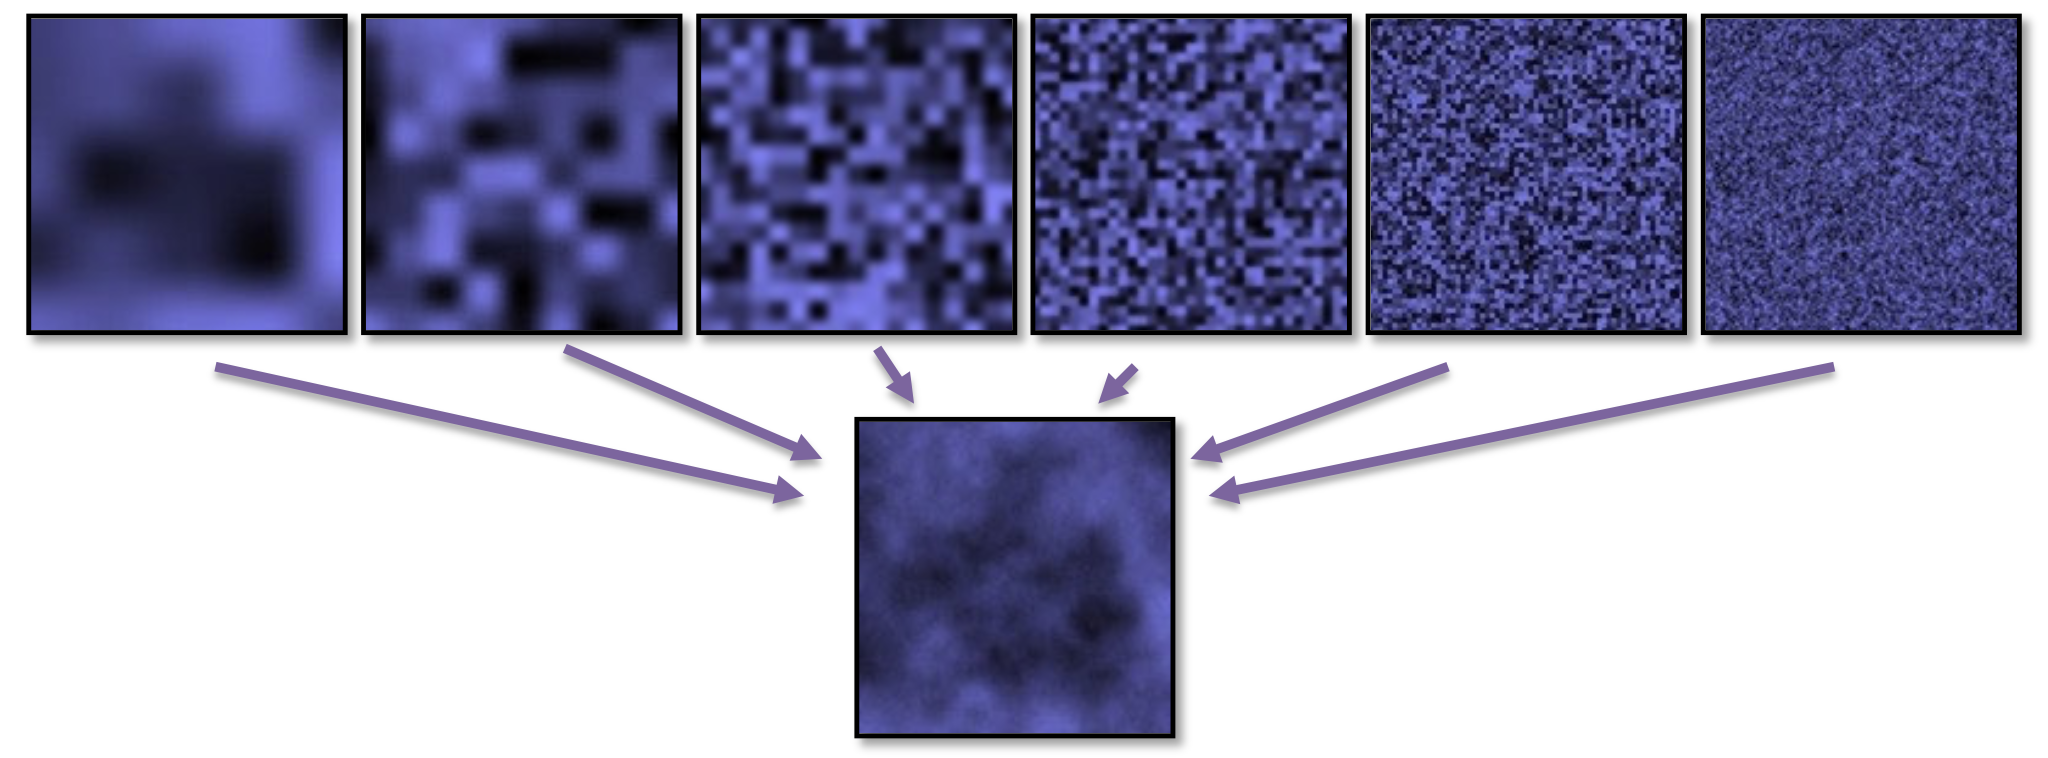
\includegraphics[width=\linewidth]{perlin_noise.png}
\end{center}
